

Uma das ferramentas, digamos externas, da qual o projecto faz uso é o {\bf md2loader}.

O md2loader é uma ferramenta de código aberto que facilmente adaptamos às nossas necessidades. Em palavras simples, existe uma classe denominada \textit{MD2Player} que permite carregar um modelo md2 e realizar operações simples como definir a escala ou render do modelo. Depois de conhecido o processo foi simples criar uma classe própria para trabalhar com a ferramenta.

\-

\begin{figure}[h]
\begin{center}
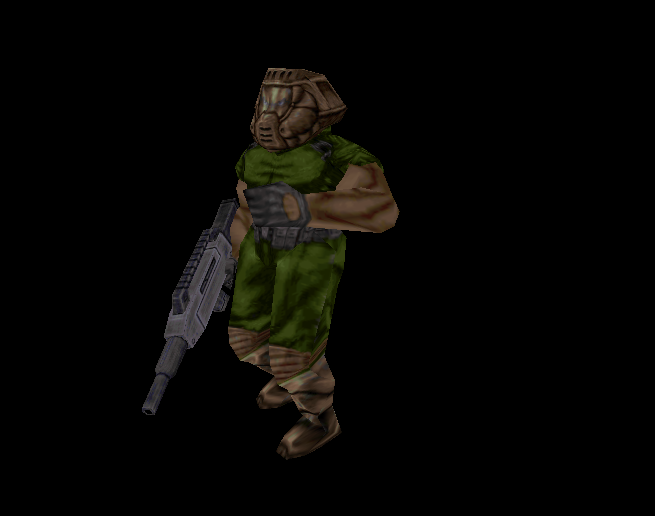
\includegraphics[width=0.5\textwidth]{images/md2loader.png}
\caption{Screenshot da ferramenta md2loader.}
\end{center}
\end{figure}



